\thispagestyle{hoccungpinone}
\pagestyle{hoccungpi}
\everymath{\color{hoccungpi}}
\graphicspath{{../hoccungpi/pic/}}
\blfootnote{\color{hoccungpi}\color{hoccungpi}$^1$...}
\begingroup
\AddToShipoutPicture*{\put(0,616){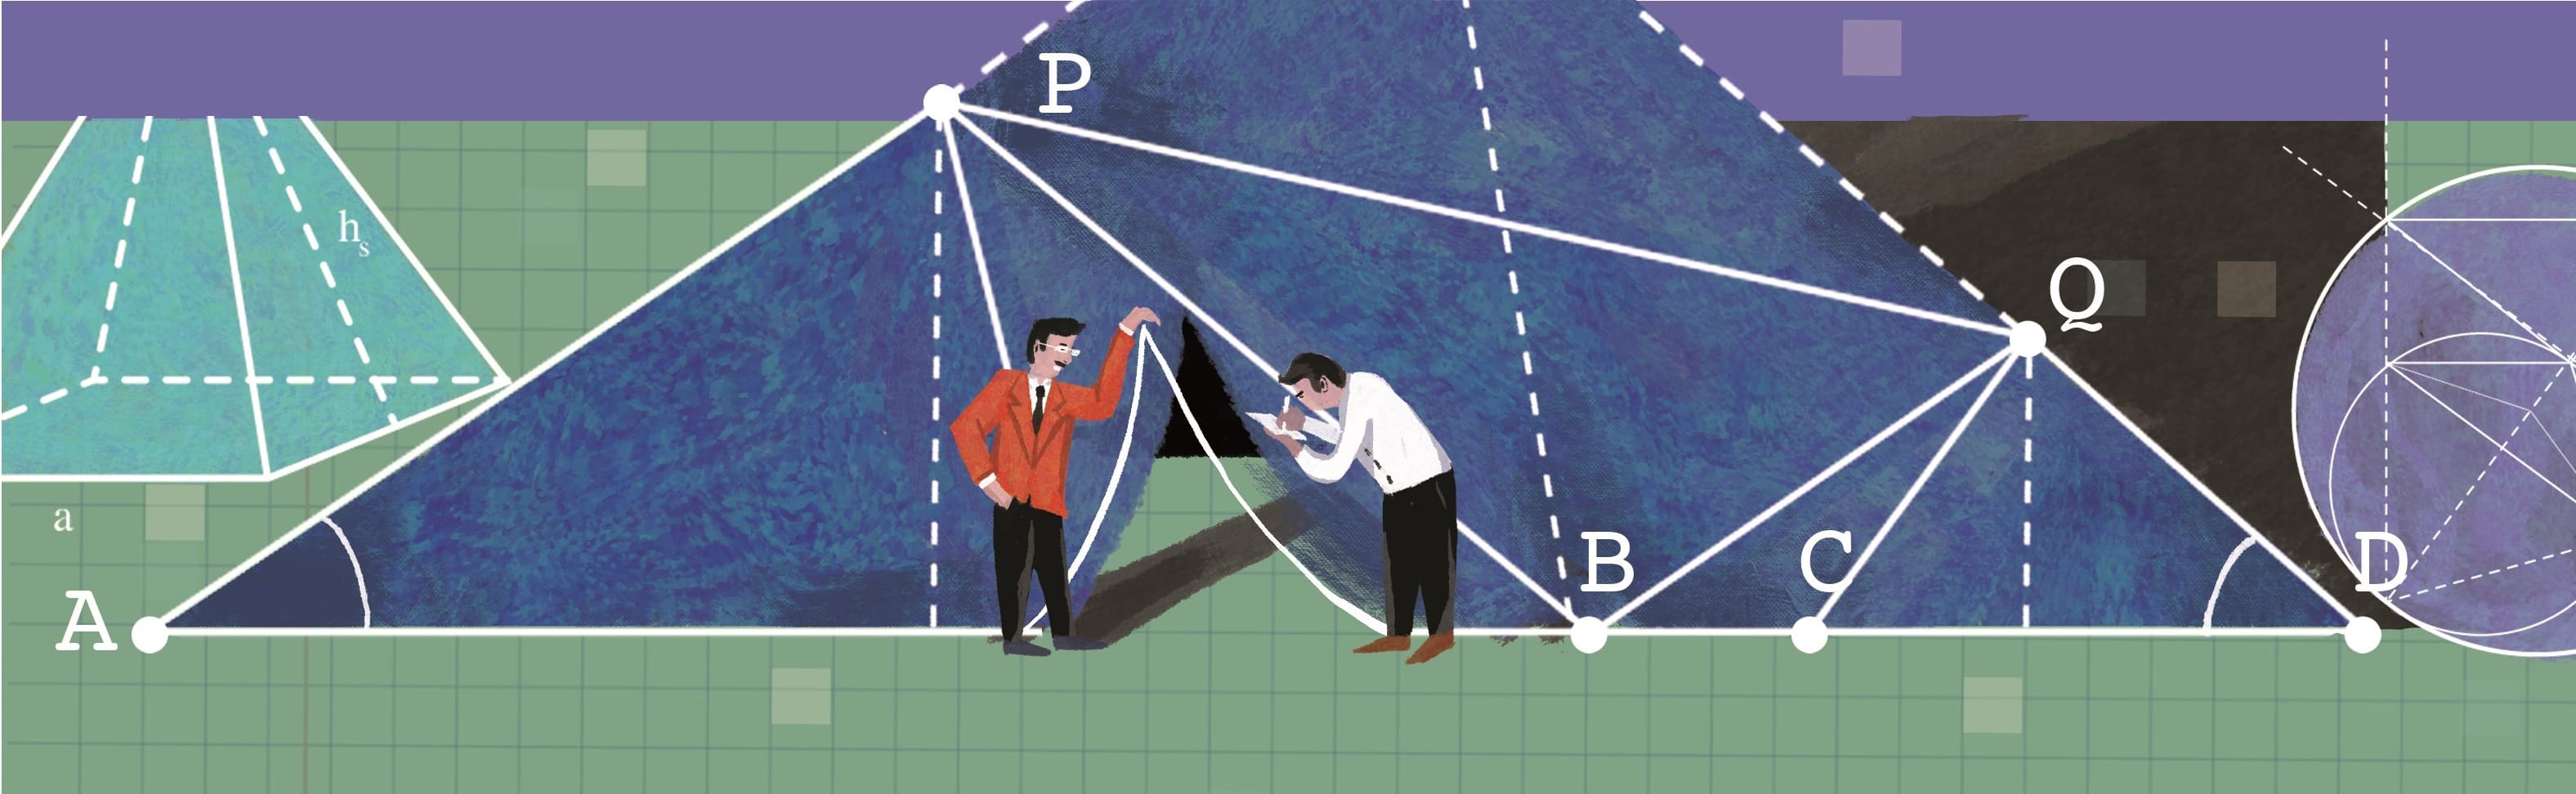
\includegraphics[width=19.3cm]{../bannerhoccungpi}}}
\AddToShipoutPicture*{\put(90,525){
\includegraphics[scale=1]{../tieude1.pdf}}}
\centering
\endgroup
\vspace*{185pt}

\begin{multicols}{2}
	Trong hành trình tìm kiếm cách làm cho môn Toán trở nên hấp dẫn hơn và gần gũi hơn đối với học sinh, việc kết hợp giữa kiến thức lý thuyết và ứng dụng là vô cùng quan trọng. Một trong những cách hiệu quả để kích thích sự quan tâm và hiểu biết của học sinh là khám phá Toán học thông qua các trò chơi. Trong bài viết này, bạn đọc sẽ được khám phá một trong những ứng dụng logic và khá thú vị của hệ nhị phân trong trò chơi đoán suy nghĩ. 
	\vskip 0.1cm
	\textbf{\color{hoccungpi}Trò chơi đoán suy nghĩ -- mục đích và các bước tiến hành}
	\vskip 0.1cm
	Trò chơi được bắt đầu bằng việc Ảo thuật gia yêu cầu Người chơi chọn một trong số $32$ lá cờ của các nước đã chuẩn bị như hình dưới đây.  Người chơi sẽ không nói cho Ảo thuật gia biết lá cờ được chọn. Nhiệm vụ của Ảo thuật gia là đoán đúng lá cờ mà Người chơi đã chọn. 
	\begin{figure}[H]
		\vspace*{-5pt}
		\centering
		\captionsetup{labelformat= empty, justification=centering}
		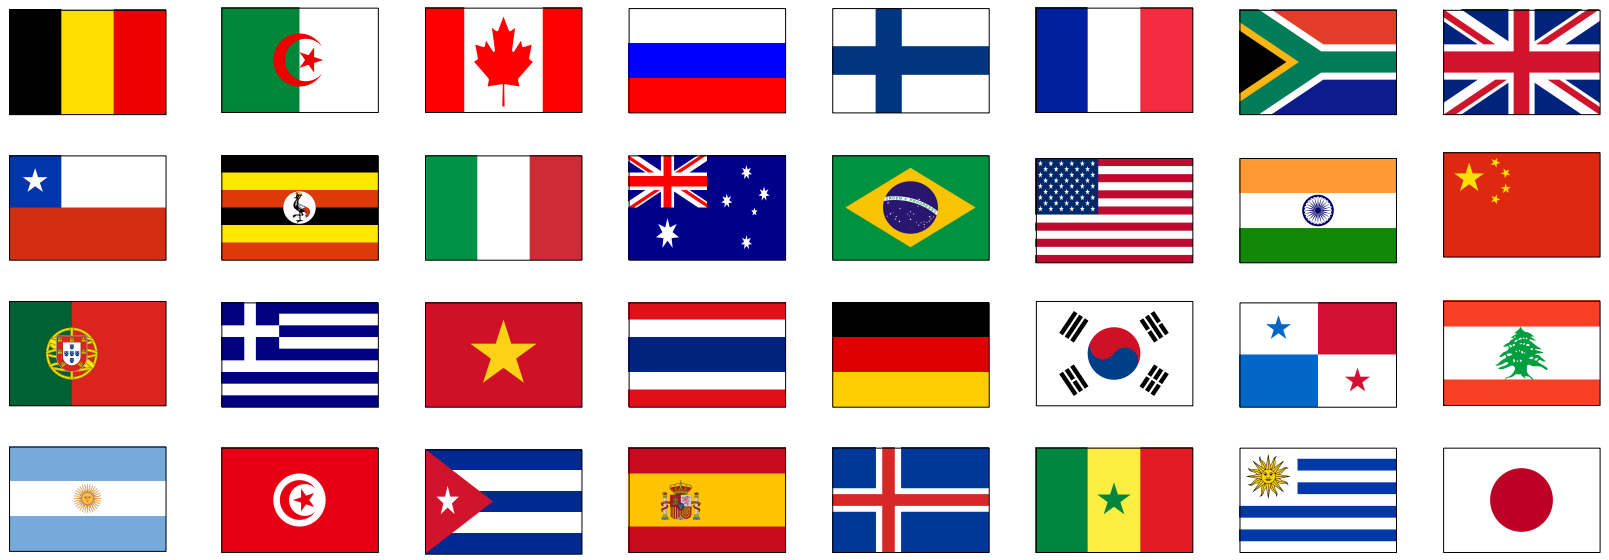
\includegraphics[width= 1\linewidth]{1}
%		\caption{\small\textit{\color{}}}
		\vspace*{-15pt}
	\end{figure}
	Để đoán đúng là cờ đã được chọn, bước tiếp theo Ảo thuật gia sẽ yêu cầu Người chơi trả lời ``Có" hoặc ``Không" cho $5$ câu hỏi dưới đây. 
	\vskip 0.1cm
	\textit{Câu hỏi $1$: Lá cờ mà bạn chọn có nằm trong dãy những lá cờ sau không?}
	\begin{figure}[H]
		\vspace*{-5pt}
		\centering
		\captionsetup{labelformat= empty, justification=centering}
		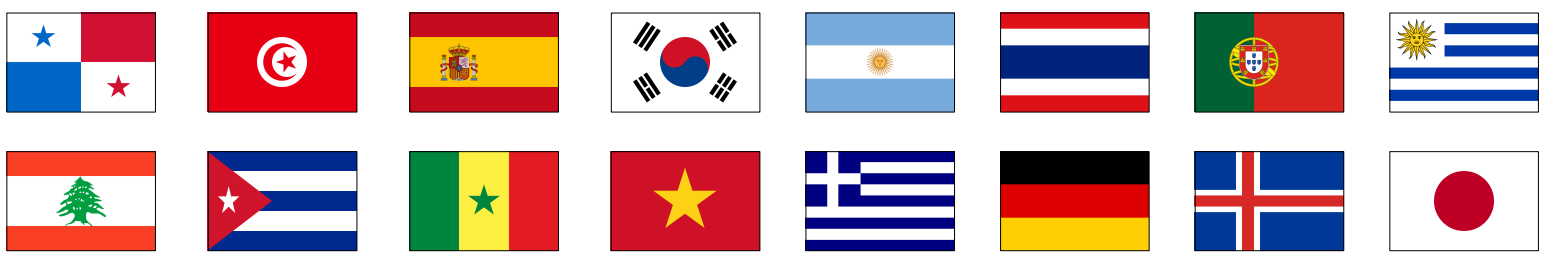
\includegraphics[width= 1\linewidth]{2}
%		\caption{\small\textit{\color{}}}
		\vspace*{-15pt}
	\end{figure}
	\textit{Câu hỏi $2$: Lá cờ mà bạn chọn có nằm trong dãy những lá cờ sau không?}
	\begin{figure}[H]
		\vspace*{-5pt}
		\centering
		\captionsetup{labelformat= empty, justification=centering}
		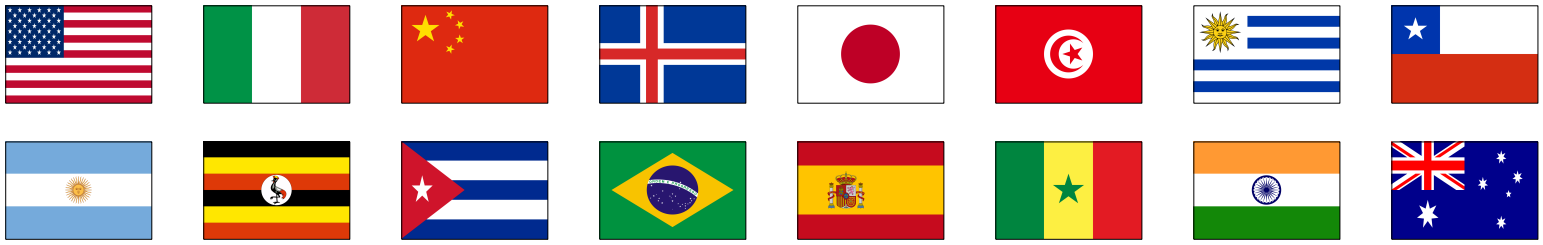
\includegraphics[width= 1\linewidth]{3}
		%		\caption{\small\textit{\color{}}}
		\vspace*{-15pt}
	\end{figure}
	\textit{Câu hỏi $3$: Lá cờ mà bạn chọn có nằm trong dãy những lá cờ sau không?}
	\begin{figure}[H]
		\vspace*{-5pt}
		\centering
		\captionsetup{labelformat= empty, justification=centering}
		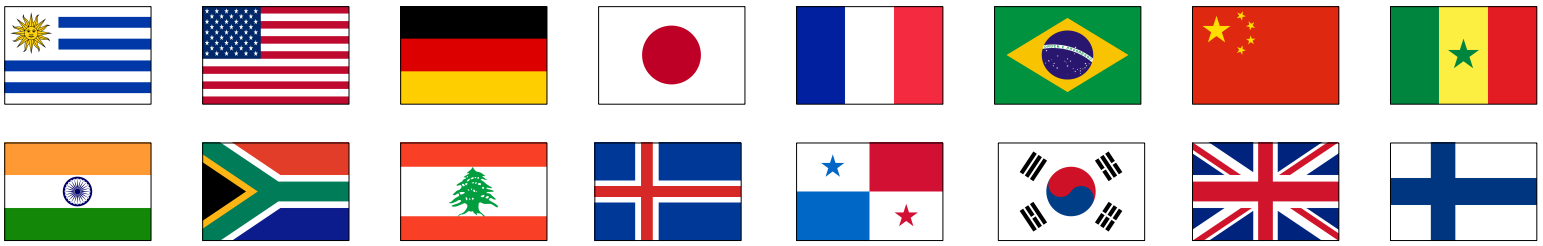
\includegraphics[width= 1\linewidth]{4}
		%		\caption{\small\textit{\color{}}}
		\vspace*{-15pt}
	\end{figure}
	\textit{Câu hỏi $4$: Lá cờ mà bạn chọn có nằm trong dãy những lá cờ sau không?}
	\begin{figure}[H]
		\vspace*{-5pt}
		\centering
		\captionsetup{labelformat= empty, justification=centering}
		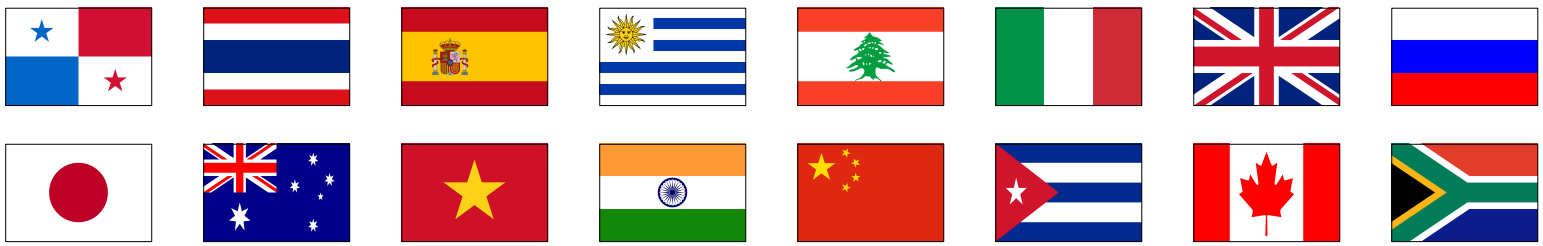
\includegraphics[width= 1\linewidth]{5}
		%		\caption{\small\textit{\color{}}}
		\vspace*{-15pt}
	\end{figure}
	\textit{Câu hỏi $s5$: Lá cờ mà bạn chọn có nằm trong dãy những lá cờ sau không?}
	\begin{figure}[H]
		\vspace*{5pt}
		\centering
		\captionsetup{labelformat= empty, justification=centering}
		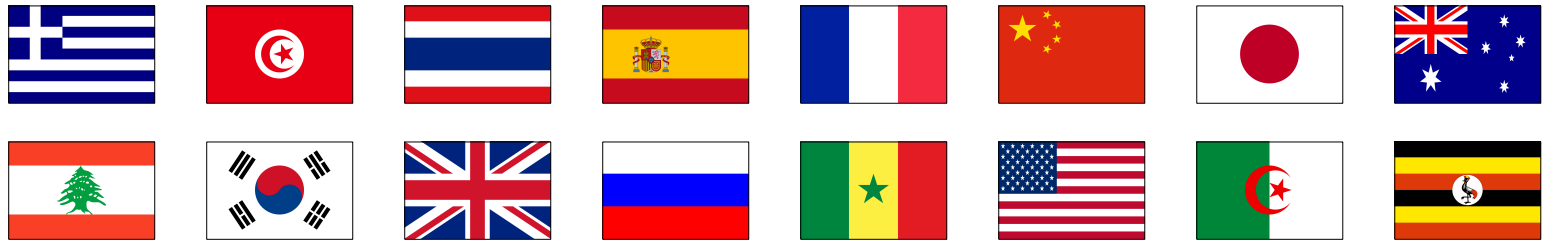
\includegraphics[width= 1\linewidth]{6}
		%		\caption{\small\textit{\color{}}}
		\vspace*{-15pt}
	\end{figure}
	Dựa vào dãy ``Có", ``Không" mà Người chơi đã đưa ra, Ảo thuật gia có thể biết một cách nhanh chóng và chính xác vị trí là cờ đã được chọn. 
	\vskip 0.1cm
	Theo bạn Ảo thuật gia đã làm thế nào? Các lá cờ trong những câu hỏi trên được chọn một cách ngẫu nhiên hay được sắp đặt sẵn? Nếu là sắp đặt sẵn thì cách chọn các lá cờ đó như thế nào? Số lượng lá cờ có ảnh hưởng tới kết quả của trò chơi? Trước khi đi trả lời một cách chi tiết, Bạn đọc hãy dành một chút thời gian suy nghĩ xem Ảo thuật gia đã làm thế nào nhé. 
	\vskip 0.1cm
	\textbf{\color{hoccungpi}Hệ nhị phân}
	\vskip 0.1cm
	Để trả lời cho những câu hỏi được nêu ra ở phần trước, trong mục này, Bạn đọc sẽ được làm quen với hệ nhị phân, cách chuyển từ hệ thập phân sang hệ nhị phân và ngược lại.
	\vskip 0.1cm
	Hệ thập phân tức hệ đếm cơ số $10$ là hệ thống số học được sử dụng phổ biến nhất trong các tính toán hàng ngày mà ở đó ta sử dụng $10$ chữ số từ $0$ đến $9$ để biểu diễn mọi số. Ví dụ như số $1234$ được biểu diễn trong hệ thập phân như sau: 
	\begin{align*}
		1234&=1\!\times\!1000\!+\!2\!\times\!100\!+\!3\!\times\!10\!+\!4\\
		&=1\!\times\! 10^3 \!+\! 2\!\times\!10^2 \!+\! 3\!\times\!10^1 \!+\! 4\!\times\!10^0.
	\end{align*}
	Tức là chữ số $1$ đại diện cho $1000$, chữ số $2$ đại diện cho $200$, chữ số $3$ đại diện cho $30$ và chữ số $4$ đại diện cho $4$ đơn vị. 
	\vskip 0.1cm
	Khác với hệ thập phân, hệ nhị phân tức hệ đếm cơ số $2$ là hệ thống số học chỉ sử dụng hai ký tự số là $0$ và $1$ để biểu diễn mọi số và mọi dữ liệu. Trong hệ nhị phân, mỗi chữ số được gọi là một ``bit", mỗi bit có thể có giá trị $0$ hoặc $1$, tương ứng với trạng thái ``tắt" và ``bật" của công tắc điện. Hệ nhị phân chính là cơ sở của hầu hết các hệ thống tính toán điện tử hiện đại do có ưu điểm tính toán đơn giản, dễ dàng thực hiện về mặt vật lý chẳng hạn như trên các mạch điện tử. Điều này khiến nó trở thành ngôn ngữ giao tiếp cơ bản giữa các thành phần của máy tính và các thiết bị điện tử khác.
	\vskip 0.1cm 
	Trong hệ nhị phân, mọi số đều biểu diễn được bằng một dãy đơn vị ``bit". Mỗi chữ số (bit) đại diện cho các bậc giá trị khác nhau, và giá trị của mỗi bit được tính dựa trên các lũy thừa của $2$. Ví dụ như số nhị phân $10101$ được biểu diễn dưới dạng tổng của các lũy thừa của $2$ như sau:
	\begin{align*}
		10101\!=\!1\!\times\!\!2^4\!+\!0\!\times\!\!2^3\!+\!1\!\times\!2^2\!+\!0\!\times\!\!2^1\!+\!1\!\!\times\!\!2^0
	\end{align*}
	tương ứng với giá trị $21$ trong hệ thập phân. 
	\vskip 0.1cm
	Để chuyển một số từ hệ thập phân sang hệ nhị phân, ta lấy số cần đổi chia với $2$ sau đó lấy kết quả chia tiếp tục với $2$, và lặp lại phép chia này cho đến khi kết quả bằng $0$. Số nhị phân thu được chính là tập hợp các số dư của các phép chia được viết theo thứ tự từ dưới lên trên. Ví dụ, để chuyển số thập phân $30$ sang hệ nhị phân ta làm như sau:
	\vskip 0.1cm 
	$\bullet$ Chia $30$ cho $2$ ta được kết quả là $15$ và số dư là $0$.
	\vskip 0.1cm
	$\bullet$ Kế tiếp, chia $15$ cho $2$ ta được kết quả là $7$ và số dư là $1$.
	\vskip 0.1cm
	$\bullet$ Ta tiếp tục chia $7$ cho $2$ thu được kết quả $3$ và số dư là $1$.
	\vskip 0.1cm
	$\bullet$ Chia $3$ cho $2$ ta được kết quả là $1$ số dư là $1$.
	\vskip 0.1cm
	$\bullet$ Chia $1$ cho $2$ ta được kết quả là $0$ và số dư là $1$. 
	\vskip 0.1cm
	Từ đó ta được biểu diễn trong hệ nhị phân của số $30$ là $11110$.
	\vskip 0.1cm 
	Ngược lại, để chuyển một số từ hệ nhị phân sang hệ thập phân ta có thể thực hiện các bước sau:
	\vskip 0.1cm 
	\textit{Bước $1$:} Viết số nhị phân thành một dãy các ký tự $0$ và $1$.
	\vskip 0.1cm
	\textit{Bước $2$:} Theo thứ tự từ trái qua phải, viết các lũy thừa của $2$ tương ứng với các chữ số, bắt đầu từ $2^0$ rồi tới $2^1\ldots$ cho đến hết.
	\vskip 0.1cm
	\textit{Bước $3$:} Tính các giá trị lũy thừa của $2$ vừa lập ra. 
	\vskip 0.1cm
	\textit{Bước $4$:}  Bỏ đi các giá trị tương ứng với vị trí số $0$, giữ lại các giá trị tương ứng với vị trí số $1$. Cộng các giá trị đó lại với nhau ta được kết quả chính là giá trị thập phân tương ứng của số nhị phân.
	\vskip 0.1cm
	Ví dụ, để tìm biểu diễn trong hệ thập phân của số nhị phân $10101$, ta lập bảng sau:
	\begin{table}[H]
		\vspace*{-5pt}
		\centering
		\captionsetup{labelformat= empty, justification=centering}
		\renewcommand{\arraystretch}{1.3}
		\setlength{\tabcolsep}{9pt}
		\begin{tabular}{|c|c|c|c|c|c|}
			\hline
			Bước $1$&	$1$	&$0$&	$1$&	$0$&	$1$\\
			\hline
			Bước $2$&	$2^4$&	$2^3$&	$2^2$&	$2^1$&	$2^0$\\
			\hline
			Bước $3$&	$16$&	$8$&	$4$&	$2$&	$1$\\
			\hline
			Bước $4$&	$16$&	X&	$4$	&X	&$1$\\
			\hline
		\end{tabular}
		\vspace*{-5pt}
	\end{table}
	Giá trị thập phân của số nhị phân $10101$ là $16+4+1=21$.
	\vskip 0.1cm 
	Bằng cách thực hiện các phương pháp nêu trên, ta dễ dàng thu được bảng chuyển đổi từ hệ thập phân sang hệ nhị phân của $32$ số tự nhiên đầu tiên như sau:
	\begin{table}[H]
		\vspace*{-5pt}
		\centering
		\captionsetup{labelformat= empty, justification=centering}
		\renewcommand{\arraystretch}{1.3}
		\resizebox{\columnwidth}{!}{\begin{tabular}{|c|c|c|c|}
			\hline
			\makecell{Hệ\\thập phân} & \makecell{Hệ\\nhị phân} & \makecell{Hệ\\thập phân} & \makecell{Hệ\\nhị phân}\\
			\hline
			$0$& $0$& $16$& $10000$\\
			\hline
			$1$& $1$& $17$& $10001$\\
			\hline
			$2$& $10$& $18$& $10010$\\
			\hline
			$3$& $11$& $19$& $10011$\\
			\hline
			$4$& $100$& $20$& $10100$\\
			\hline
			$5$& $101$& $21$& $10101$\\
			\hline
			$6$& $110$& $22$& $10110$\\
			\hline
			$7$& $111$& $23$& $10111$\\
			\hline
			$7$& $1000$& $24$& $11000$\\
			\hline
			$9$& $1001$& $25$&$11001$\\
			\hline
			$10$& $1010$& $26$& $11010$\\
			\hline
			$11$& $1011$& $27$& $11011$\\
			\hline
			$12$& $1100$& $28$& $11100$\\
			\hline
			$13$ &$1101$& $29$& $11101$\\
			\hline
			$14$& $1110$& $30$& $11110$\\
			\hline
			$15$& $1111$& $31$& $11111$\\
			\hline 
		\end{tabular}}
%		\vspace*{-5pt}
	\end{table}
	\textbf{\color{hoccungpi}Bí mật của trò chơi đoán suy nghĩ}
	\vskip 0.1cm 
	Để trả lời câu hỏi Ảo thuật gia đã làm thế nào, ta đánh số các lá cờ từ $0$ tới $31$ như hình dưới đây.
	\begin{figure}[H]
		\vspace*{-5pt}
		\centering
		\captionsetup{labelformat= empty, justification=centering}
		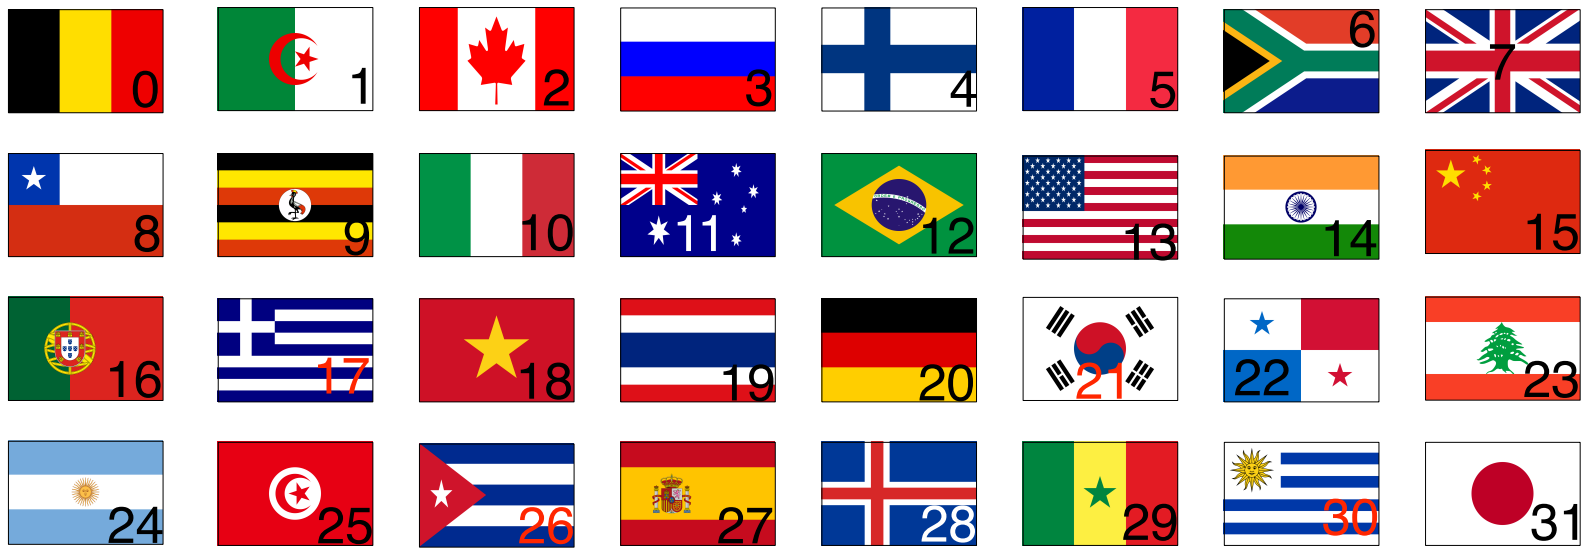
\includegraphics[width= 1\linewidth]{7}
%		\caption{\small\textit{\color{}}}
		\vspace*{-15pt}
	\end{figure}
	Bí mật của trò chơi đoán suy nghĩ nằm ở biểu diễn trong hệ nhị phân của giá trị của mỗi lá cờ trên. Tưởng tượng rằng Người chơi chọn lá cờ của Việt Nam. Sau khi trả lời $5$ câu hỏi của Ảo thuật gia, ta thu được dãy câu trả lời như sau: Có -- Không -- Không -- Có -- Không . Ảo thuật gia sẽ thay thế từ ``Có" bởi số $1$ và từ ``Không" bởi số $0$ để nhận được biểu diễn trong hệ nhị phân như sau: $10010$. Bằng cách chuyển số đó qua hệ thập phân, Ảo thuật gia thu được kết quả là $18$ (xem ở bảng dưới đây) -- tương ứng với vị trí của là cờ của nước Việt nam như đã đánh số ban đầu.
	\vskip 0.1cm
	\begin{table}[H]
		\vspace*{-5pt}
		\centering
		\captionsetup{labelformat= empty, justification=centering}
		\renewcommand{\arraystretch}{1.35}
		\resizebox{\columnwidth}{!}{\begin{tabular}{|l|c|c|c|c|c|}
			\hline
			\makecell{Dãy câu\\ trả lời}&	Có&	Không&	Không&	Có&	Không\\
			\hline
			\makecell{Hệ\\nhị phân}&	$1$&	$0$&	$0$&	$1$&	$0$\\
			\hline
			\makecell{Lũy thừa\\ $2$}&	$2^4$&	$2^3$&	$2^2$&	$2^1$&	$2^0$\\
			\hline
			\makecell{Giá trị\\ tương ứng}&	$16$&	X&	X&	$2$&	X\\
			\hline
			\multicolumn{6}{|l|}{\makecell[c]{Giá trị trong hệ thập phân nhận được là $16+2=18$\\ tương ứng với vị trí của lá cờ được chọn trong bảng\\ các lá cờ được đưa ra ban đầu.}}\\
			\hline
		\end{tabular}}
%		\vspace*{-5pt}
	\end{table}
	Đến đây Bạn đọc có thể dễ dàng nhận thấy rằng việc chọn các lá cờ trong $5$ câu hỏi mà Ảo thuật gia đã  đưa ra ban đầu là không ngẫu nhiên. Sự lựa chọn có tính sắp đặt đó hoàn toàn phụ thuộc vào biểu diễn trong hệ nhị phân của giá trị của từng lá cờ. Ví dụ như lá cờ của Việt Nam có vị trí tương ứng là $18$, giá trị chuyển của hệ nhị phân là $10010$. Từ đó Ảo thuật gia sẽ sắp đặt sao cho lá cờ của Việt Nam chỉ xuất hiện trong câu hỏi $1$ và câu hỏi $4$. Thêm một ví dụ nữa là lá cờ của nước Canada được đánh số $2$, chuyển qua hệ nhị phân ta được $10$ hay $00010$, chính vì vậy lá cờ của Canada chỉ xuất hiện trong câu hỏi số $4$ mà không xuất hiện trong những câu hỏi còn lại. Tương tự như vậy Ảo thuật gia có thể dễ dàng sắp đặt các lá cờ còn lại trong các câu hỏi để cho việc tìm lại lá cờ được chọn diễn ra một cách chính xác và nhanh chóng. 
	\vskip 0.1cm
	\textbf{\color{hoccungpi}Tài liệu tham khảo}
	\vskip 0.1cm
	Transmission de pensée -- La magie du binaire -- Inria -- Institut national de recherche en sciences et technologies du numérique (hal. science). 
\end{multicols}